\newcommand{\deposition}{1000}

\section{Inledning}
Kontrollera alltid alla ytor och rum som ni eller era gäster har nyttjat. Ni som arrangörer är ansvariga för att \textbf{alla} områden som finns med i detta dokument kontrolleras och är rena, även om det inte är ni som har skräpat ner. Vi som arrangerar i Hubben är de enda som ser till att det är städat och det är därför viktigt att vi alla drar vårt strå till stacken så att den inte faller sönder.\\

 Dokumentet ger dock en god insikt i vad vi i P.R.I.T. anser vara ett korrekt städ och det är därför en god idé att checka av alla punkter innan städet anses färdigt.\\

Tips: Se över hur möbler står redan innan ert arrangemang, så att ni vet hur ni ska ställa tillbaka dem! (Tips: Ta bilder ifall du inte kan möbleringen). \\

Då städet är färdigt ska ni ta bilder på alla delar av Hubben för att kunna bevisa att ni faktiskt städade, skicka sedan dessa till P.R.I.T.. Det kan hända att andra personer stökar ner efter att ni har städat.\\

Kontakta P.R.I.T. (prit@chalmers.it) om ni har några frågor eller funderingar.

\section{Deposition}
\begin{itemize}
    \item En deposition på \deposition :- utgår vid bokning av Hubben 2.2 av någon som inte vid bokningstillfället är en del av Teknologsektionen Informationsteknik. (P.R.I.T. reserverar för sig vid otydlighet sista ordet i den här frågan.)
    \item Vid bristfälligt följande av bokningsvillkoren som beskrivs i detta dokument förbihåller P.R.I.T. rätten att behålla hela, eller en del av depositionen.
    \item Går dyrare inventarier sönder på grund av misskötsel kan detta komma att faktureras.
\end{itemize}

\section{Prickar}
För medlemmar i Teknologsektionen Informationsteknik så finns inte någon deposition, därför finns istället ett prick-system. 
Vid undermålig städning så kan P.R.I.T. ge den/de som har bokat en eller flera prickar beroende på det bedömda allvaret. 
Detta innefattar sektionsorganet eller den övrigt sektionsassocierade föreningens styrelse.\\
När man fått tre prickar så får man inte boka Hubben förrän man blivit av med alla dessa.
För att bli av med prickar så kan man bli ombedd att hjälpa P.R.I.T. med diverse uppgifter i Hubben. Detta går göra även om man inte har tre prickar.
Några exempel på vad P.R.I.T. kan be er att göra är: 
\begin{itemize}
    \item Rengöra microvågsugnarna.
    \item Rengöra kylar och frysar i köket.
\end{itemize}
Om ens sektionsorgan eller sektionsassocierade förening är stoppad från att boka så får man inte boka CTC eller Grupprummet som enskild person. Man får inte heller stå som ansvarig för något annat sektionsorgan eller sektionsassocierade förenings bokning.
\section{Allmänt}
Dessa saker görs ofta sist.
\begin{itemize}
    \item Se till att alla moppar är rengjorda och torra, tvätta dem i rent vatten i en skurhink och krama ur dem.
    \item Se till att städinventarier är på rätt plats och att de är rena.
    \item Släck alla lampor i Hubben (glöm inte hallen och toaletterna).
    \item Stäng alla fönster i Hubben.
    \item Stäng av och töm kylarna bakom baren. Se till att de lämnas på glänt, annars börjar det lukta illa! Detta gäller även frysen längst in i baren. 
    \item Töm alla sopor.
    \item Soprummet för brännbart ligger på hörsalsvägen, förbi ingången till EDIT-innergården på högersidan, nyckeln ligger längst in till vänster på mittersta hyllan i städskåpet. Se röd prick på kartan nedan.
    \item Glaskärl finns på Elektroinnergården. Se grön prick på kartan nedan.
    \item Resterande sopor slängs i det nordvästra soprummet i EDIT-huset (om du inte har access till Guldgruvan, meddela P.R.I.T.). Det är viktigt att allt sorteras korrekt! 
    \subitem - Töm plaståtervinning om den är full.
    \subitem - Töm kartongåtervinning om den är full.
    \subitem - Töm glasåtervinning om den är full.
    \subitem - Töm metallåtervinning om den är full.
    \subitem - Töm alla brännbara sopor om de är fulla eller luktar illa. Detta är särskilt viktigt under ledigheter eftersom ni då är de enda som tömmer. 
    
\end{itemize}


\section{Stor-Hubben och hallen}
\begin{itemize}
    \item Tänd de starka lamporna med knappen bredvid baren eller vid toaletterna så att ni ser ordentligt.
    \item Torka av alla bord, stolar och soffor.
    \item Flytta möblerna till studierummet innan ni gör rent golvet.
    \item Rengör golvet.
    \begin{itemize}
        \item Sopa golvet.
        \item Upprepa tills golvet anses rent (vanligtvis en eller två gånger):
        \begin{enumerate}
            \item Moppa golvet med endast varmvatten (använd bara medel om det är fettfläckar som inte går bort efter två vattenmoppningar). Kranen i köket är enklast att fylla på vid samt ger varmast vatten.
            \item Raka golvet.
            \item Töm mopphinkar så fort botten inte syns. Töm i toaletten och spola.
        \end{enumerate}
        \item Moppa tunnt med lite vatten en sista gång och låt det lufttorka (för att undvika märken från rakor).
        \item Töm mopphinkarna i toaletten och spola. Skölj även ur mopphinkarna med vatten en sista gång.
    \end{itemize}
    \item Bär tillbaka alla möblerna och placera dem som de stod innan arrangemanget.
    \item Stäng av projektor och se till att bardatorn inte spelar musik.
    \item Torka av och gör rent bardisken.
    \item Dra upp persiennerna.
\end{itemize}

\section{Köket}
\begin{itemize}
    \item Diska all disk, starta diskmaskinen.
    \item Torka av stekplattor (inklusive sladdarna), köksytor och bord med vatten och städmedel.
    \item Rengör golvet.
    \begin{itemize}
        \item Sopa golvet.
        \item Upprepa tills golvet anses rent (vanligtvis en eller två gånger):
        \begin{enumerate}
            \item Moppa golvet med endast varmvatten (använd bara medel om det är fettfläckar som inte går bort efter två vattenmoppningar). Kranen i köket är enklast att fylla på vid samt ger varmast vatten.
            \item Raka golvet.
            \item Töm mopphinkar så fort botten inte syns. Töm i toaletten och spola.
        \end{enumerate}
        \item Töm mopphinkarna i toaletten och spola. Skölj även ur mopphinkarna med vatten en sista gång.
    \end{itemize}
    \item Töm diskstället och diskmaskinen (om diskmaskinen inte är klar, töm den innan lunch dagen efter).
\end{itemize}

\section{Grupprummet}
\begin{itemize}
    \item Torka av alla bord.
    \item Placera möblerna som de stod innan arrangemanget.
    \item Dra upp persiennerna i fönstrena mellan stor-Hubben och Grupprummet.
    \item Sopa golvet.
    \item Vid behov, moppa golvet på samma sätt som i stor-Hubben.
    \item Vid behov, rengör whiteboardtavlan
\end{itemize}

\section{Studierummet}
\begin{itemize}
    \item Sopa golvet.
    \item Sätt tillbaka alla möbler till så som de var innan arrangemanget. Se till att alla överblivna stolar står staplade i en enda stapel mot väggen.
\end{itemize}

\section{Toaletter och områden utanför Hubben}
Vanligtvis behöver det inte städas utanför, men det är ändå viktigt att kontrollera att ert arrangemang inte har stökat ner.
\subsection{Toaletter}
Notera att det här gäller alla tre toaletterna inne i Hubben samt vid behov de två utanför E-Studion.
\begin{itemize}
    \item Kontrollera att det inte finns någon spya, toalettpapper, snus eller annat äckligt på golvet.
    \item Se till att det inte är stopp i någon av toaletterna (testa genom att spola). Om det är det så kan det lösas med hjälp av vaskrensaren under diskhon i köket (rengör den efter användning).
    \item Töm soporna ifall de är fulla eller luktar illa.
    \item Rengör handfat och toalett med papper och städmedel.
    \item Rengör på väggar och spegel vid behov.  
    \item Sopa och moppa golvet.
\end{itemize}

\subsection{Utanför E-Studion}
\begin{itemize}
    \item Sopa golvet om det är smutsigt.
    \item Moppa golvet om det är kletigt.
    \item Torka av bord, bänkar och fönsterbleck.
    \item Se till att alla möbler är placerade som de ska.
\end{itemize}

\subsection{Hörsalsvägen}
Det är väldigt sällan det faktiskt behövs göras något utanför byggnaden, men ta en snabb titt så att det inte finns några burkar, fimpar, spya, etc. Allra viktigast är trappan och rampen precis utanför entrén.

\newpage
\section{Karta över Hubben med omnejd}
Hjärta: Hubben. Cirkel: Soprum för brännbart. Triangel: Glaskross och Guldgruvan. Kvadrat: Återvinningscentral
\begin{figure}[h]
    \centering
    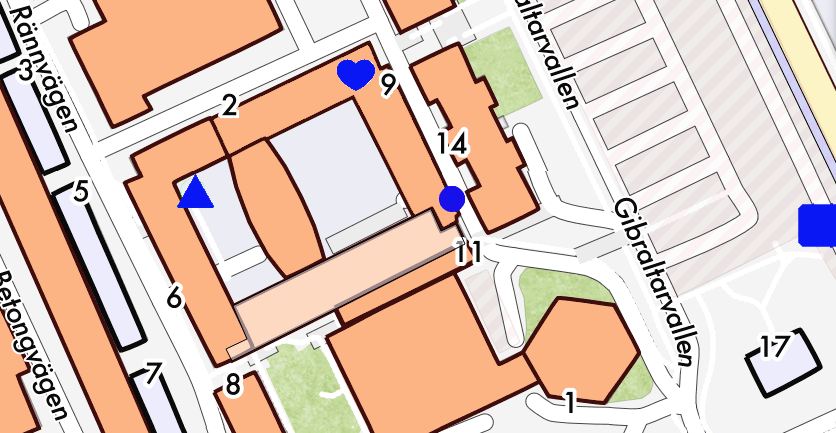
\includegraphics[scale=0.5, angle=0]{epic_map}
    \label{fig:map}
\end{figure}
